%% This skeleton file requires IEEEtran.cls version 1.6 or later.
%%
\documentclass[conference,letterpaper]{IEEEtran}
% If the IEEEtran.cls has not been installed into the LaTeX system files,
% manually specify the path to it:
% \documentclass[conference]{../sty/IEEEtran}
\IEEEoverridecommandlockouts
\overrideIEEEmargins

% some very useful LaTeX packages include:

%\usepackage{cite}      % Written by Donald Arseneau
                        % V1.6 and later of IEEEtran pre-defines the format
                        % of the cite.sty package \cite{} output to follow
                        % that of IEEE. Loading the cite package will
                        % result in citation numbers being automatically
                        % sorted and properly "ranged". i.e.,
                        % [1], [9], [2], [7], [5], [6]
                        % (without using cite.sty)
                        % will become:
                        % [1], [2], [5]--[7], [9] (using cite.sty)
                        % cite.sty's \cite will automatically add leading
                        % space, if needed. Use cite.sty's noadjust option
                        % (cite.sty V3.8 and later) if you want to turn this
                        % off. cite.sty is already installed on most LaTeX
                        % systems. The latest version can be obtained at:
                        % http://www.ctan.org/tex-archive/macros/latex/contrib/supported/cite/

\usepackage[dvips]{graphicx}  % Written by David Carlisle and Sebastian Rahtz
                        % Required if you want graphics, photos, etc.
                        % graphicx.sty is already installed on most LaTeX
                        % systems. The latest version and documentation can
                        % be obtained at:
                        % http://www.ctan.org/tex-archive/macros/latex/required/graphics/
                        % Another good source of documentation is "Using
                        % Imported Graphics in LaTeX2e" by Keith Reckdahl
                        % which can be found as esplatex.ps and epslatex.pdf
                        % at: http://www.ctan.org/tex-archive/info/

%\usepackage{amsmath}   % From the American Mathematical Society
                        % A popular package that provides many helpful commands
                        % for dealing with mathematics. Note that the AMSmath
                        % package sets \interdisplaylinepenalty to 10000 thus
                        % preventing page breaks from occurring within multiline
                        % equations. Use:
\usepackage{multirow}
\usepackage[left=0.71in,top=0.94in,right=0.71in,bottom=1.18in]{geometry}
\setlength{\columnsep}{0.24in}
% correct bad hyphenation here
%\hyphenation{op-tical net-works semi-conduc-tor IEEEtran}


\begin{document}
% paper title
\title{\huge Simultaneous Coordinate Calibrations by Solving the AX=YB Problem without Correspondence $^{*}$\footnoterule\thanks{$^{*}$This work is partially
supported by NSF Grant RI-Medium: \#IIS-1162095 to }}

% author names and affiliations
\author{\authorblockN{Haiyuan Li}
\authorblockA{\textit{School of Mechanical Engineering}\\
\textit{Beihang University}\\
\textit{Beijing, China}\\
\textit{lihaiyuan@buaa.edu.cn}\\}%
\and
\authorblockN{Gregory S. Chirikjian}
\authorblockA{\textit{Department of Intelligent Robotics}\\
\textit{Johns Hopkins University}\\
\textit{Baltimore, Maryland, USA}\\
\textit{gregc@jhu.edu}\\}}%

% make the title area
\maketitle
\begin{abstract}

\\
\end{abstract}

% key words
\begin{keywords}
AX=YB, Sensor Calibration, Probabilistic Modeling
\end{keywords}

\section{Introduction}
% no \PARstart

Image-guided system has been widely used in robotics such as robot assisted surgery. Sensors such as a camera, a laser scanner and an ultrasound probe are usually mounted as the end-effector of a robotic manipulator. For a typical ``hand-eye" system as described above, the relative transformation of the sensor with respect to the end-effector should be accurately calibrated, and it is often characterized as the well known $\textbf{AX=XB}$ problem. A variation of this problem is characterized as the $\textbf{AX=YB}$ problem, where both the hand-eye transformation and the pose of the robot base with respect to the world frame need to be calibrated. In a typical environment setup, the relationship among the sensor frame, robot frame and world frame either is subject to change or can be disturbed by uncertainties. Therefore, simultaneous coordinate calibrations have to be performed frequently in order to enable the robot to respond to dynamic environments.

In the $\textbf{AX=YB}$ problem, $A$s and $B$s can be respectively obtained via different sensors. The data streams can be in an asynchronous fashion due to different working frequencies of the sensors. The asynchrony causes a shift between the two streams of data which damages the correspondence between $A$s and $B$s. In this paper, we present a method to solve for $X$ and $Y$ without the need to know a priori knowledge of the correspondence between $A$s and $B$s.

\begin{center}
\begin{figure}[htbp]
\centering
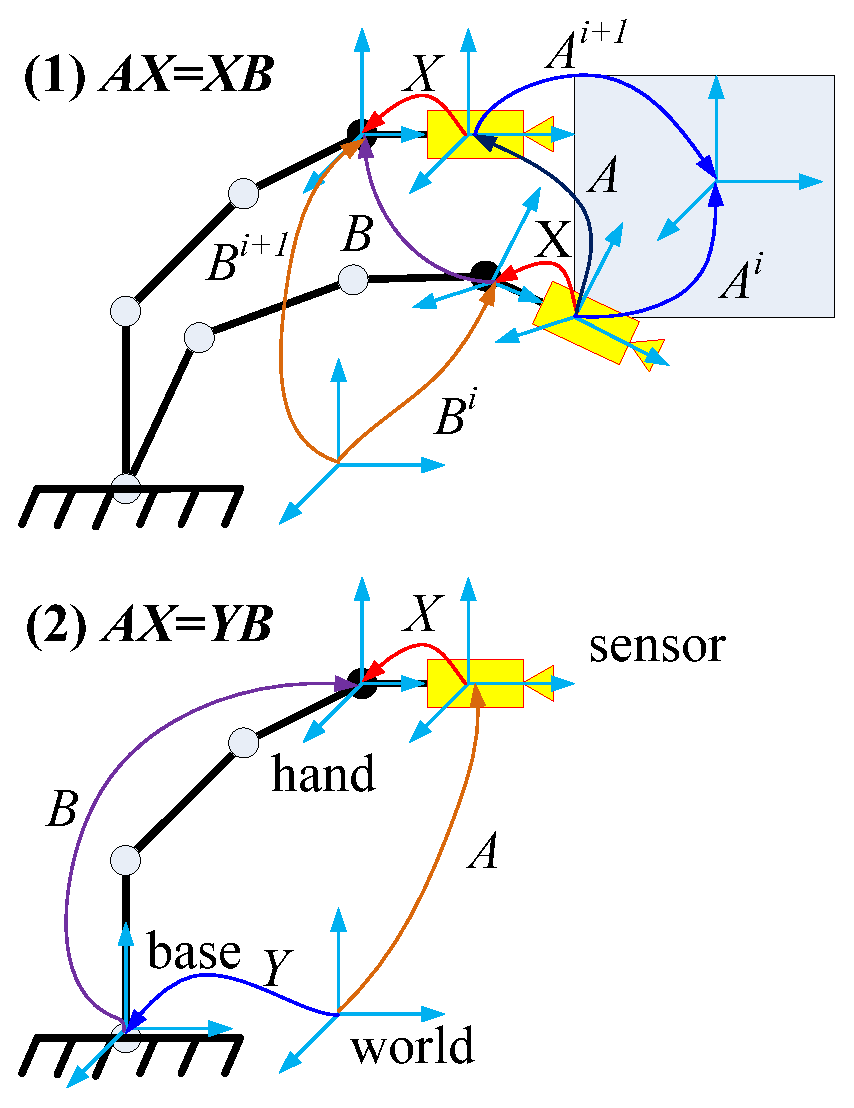
\includegraphics[width=2in]{fig1.eps}
\caption{
(1) The hand-eye calibration problem formulated in a matrix as AX=XB. (2) The hand-eye and robot-robot calibration problem formulated as AX=YB.
}
\label{fig1}
\end{figure}
\end{center}

The hand-eye calibration problem can be modeled as the $\textbf{AX = XB}$, where $A$s and $B$s are the homogeneous transformation matrices describing the relative motion of the end-effector and the sensor respectively. As shown in Fig.~\ref{fig1}, $A = A^{i}(A^{i+1})^{-1}$ and $B = B^{i}(B^{i+1})^{-1}$. The homogeneous transformation matrix can be described as:
\begin{equation}\label{equ0}
    g(R,t)=\left(
             \begin{array}{cc}
               R & t \\
               0^{T} & 1 \\
             \end{array}
           \right)
\end{equation}

where $R \in SO(3)$ is a rotation matrix and $t \in R^{3}$ is a translation vector.

Given multiple pairs of $(A_{i},B_{i}) \in SE(3) \times SE(3)$ with correspondence, many methods have been proposed to solve for $X$ including decoupling of rotation and translation, least squares fitting, singular value decomposition (\emph{SVD}), screw theory, nonlinear
optimization, quaternion, gradient descent and interactive approaches \cite{Shiu1989,Tsai1989,Wang1992,Park1994,Horaud1995,Daniilidis1999,Fassi2005,Zhao2011,Ackerman2014a}. Theses methods assume that there is exact knowledge of the $As$ and $Bs$ correspondence. Considering data streams containing the $A$ and $B$ will be asynchronous that are discussed in many instances
in the literature, several methods regardless of the correspondence or recovering the correspondence between two data sets are presented \cite{Ackerman2013a,Ackerman2013,Ackerman2014}.

Simultaneous estimation of the hand-eye transformation and robot-world one
has been viewed as $\textbf{AX=YB}$ problem. As shown in Fig.~\ref{fig1}, $Y$ is the transformation of the robot base relative to the world, $A$ is the sensor to the world transformation, and $B$ is the hand/end-effector to the robot base rigid transformation. The $A$ and $B$ in $\textbf{AX=YB}$ calibration is different from ones in $\textbf{AX=XB}$ from a physical view. This problem has been studied in different methods such as SVD, closed-form, quaternion and nonlinear optimization \cite{Zhuang1994,dornaika1998simultaneous,Hirsh2001, ernst2012non,strobl2006optimal,Li2010,Shah2013,Heller2014}. Another approach integrate multiple robots to calibrate hand-eye, tool-flange and robot-robot transformation in $\textbf{AXB=YCZ}$ problem \cite{Wang2014}. Simultaneous solution for $X$ and $Y$ in $\textbf{AX=YB}$ problem is an challenging issue. In the above methods, the correspondence between $A$ and $B$ is known a prior. In this paper, our solution for $\textbf{AX=YB}$ doesn't require a priori knowledge of correspondences.

The rest of the paper is organized as follows. In Section
\ref{sect2} we present the probabilistic theory to solve for $X$ and $Y$. In Section \ref{sect3} a algorithmic solution involving correlation theorem and Euclidean group invariants is posed to recover the correspondence. The simulation results, including known  and unknown correspondence, are illustrated in Section \ref{sect4}. Finally, we draw some conclusions.

\section{Solving AX=YB using a probabilistic theory on motion groups}
\label{sect2}

Given a large set of pairs $(A_{i},B_{i})\in SE(3)\times SE(3)$ for $i=1,\cdots,n$ that are acquired by measurements and satisfy the following equations

\begin{equation}\label{equ1}
A_{i}X=YB_{i}
\end{equation}

In the case of $SE(3)$, a Dirac delta function, or $\delta$ function, is thought of as a function which is zero everywhere except at the identity where it is infinite.

\begin{equation}\label{equ2}
\delta{(H)}=
\left\{
\begin{array}{ll}
+\infty, & H=I \\
0, & H \neq I
\end{array}
\right.
\end{equation}

Dirac delta function is also constrained to satisfy the identity.

\begin{equation}\label{equ3}
\int_{SE(3)}\delta{(H)}dH=1
\end{equation}

A shifted Dirac delta function can be defined as $\delta_{A}(H)=\delta{(A^{-1}H)}$. Given two functions $f_{1}(g)$ and $f_{2}(g)$, their convolution in Lie group is defined as follows,

\begin{equation}\label{equ4}
(f_{1}\ast f_{2})(g)=\int_{SE(3)}f_{1}(h)f_{2}(h^{-1}\circ g)dh
\end{equation}

Considering the properties of $\delta$ function, the following equation is built.

\begin{equation}\label{equ5}
(f\ast \delta)(g)=\int_{SE(3)}f(h)\delta(h^{-1}\circ g)dh=f(g)
\end{equation}

Therefore, for each $A_{i}$ and $B_{i}$ can get

\begin{IEEEeqnarray}{l}\label{equ6}
(\delta_{A_{i}}\ast \delta_{X})(g)=\delta(A_{i}^{-1} g X^{-1}) \IEEEyessubnumber
\\*
(\delta_{Y}\ast \delta_{B_{i}})(g)=\delta(Y^{-1} g B_{i}^{-1}) \IEEEyessubnumber
\end{IEEEeqnarray}

Together with $g=A_{i}X=YB_{i}$, we can obtain the convolution equation

\begin{equation}\label{equ7}
(\delta_{A_{i}}\ast \delta_{X})(g)=(\delta_{Y}\ast \delta_{B_{i}})(g)
\end{equation}

Convolution provides a linear operation on functions with additional properties. We can add up $n$ instances into a single function.

\begin{IEEEeqnarray}{l}\label{equ8}
f_{A}(g)=\frac{1}{n}\sum_{i=1}^{n} \delta(A_{i}^{-1}g) \IEEEyessubnumber
\\*
f_{B}(g)=\frac{1}{n}\sum_{i=1}^{n} \delta(B_{i}^{-1}g) \IEEEyessubnumber
\end{IEEEeqnarray}

Therefore,

\begin{equation}\label{equ9}
(f_{A_{i}}\ast \delta_{X})(g)=(\delta_{Y}\ast f_{B_{i}})(g)
\end{equation}

In each transformation set $A_i$s and $B_i$s, we are using small relative motions between consecutive reference frames. Given a measure of distance between reference frames, e.g.

\begin{eqnarray}\label{equ10}
d^{2}(A_{i},A_{j})=\parallel \Delta A \parallel_{W}^{2} = trace[(\Delta A)W(\Delta A)^{T}] = \epsilon,\nonumber \\
\end{eqnarray}

we have that  $\Delta A = A_{i}-A_{j}$ and $0 < \epsilon \ll 1 $

The convolution of "highly focused" distributions corresponding to closely clumped sets of reference frames have some interesting properties that we can exploit to solve for $X$. In particular, let the mean and covariance of a probability density, $f(g)$(e.g. $f_{A}(g),f_{B}(g)$), be defined by the conditions.


\begin{IEEEeqnarray}{l}\label{equ11}
\int_{SE(3)}log(M^{-1}g))f(g)dg=0 \IEEEyessubnumber
\\*
\Sigma = \int_{SE(3)}log^{\vee}(M^{-1}g)[log^{\vee}(M^{-1)}g)]^{T}f(g)dg \IEEEyessubnumber
\end{IEEEeqnarray}

A discrete version as for $f_{A}(g)$ is

\begin{IEEEeqnarray}{l}\label{equ12}
\sum_{i=1}^{n}log(M^{-1}g))=0 \IEEEyessubnumber
\\*
\Sigma_{A} = \sum_{i=1}^{n}log^{\vee}(M^{-1}g)[log^{\vee}(M^{-1)}g)]^{T} \IEEEyessubnumber
\end{IEEEeqnarray}

While the cloud of frames ${A_{i}}$ is clustered around $M_{A}$, an iterative formula can be used for computing $M_{A}$ \cite{Wang2008}.

\begin{equation}\label{equ13}
    ^{k+1}M_{A} = ^{k}M_{A} \circ exp[\frac{1}{n}\sum_{i=1}^{n}log(^{k}M_{A}^{-1}\circ A_{i})]
\end{equation}

An initial estimate of the iterative procedure can be $^{0}M_{A}=\frac{1}{n}\sum_{i=1}^{n}log(A_{i})$,then the process iterates until the cost function, $\parallel \sum_{i=1}^{n}log(M_{A}^{-1}A_{i}) \parallel^{2}$ falls below a predefined threshold, where the cost function is minimized and the minimum defines $M_{A}$. A similar procedure is used for computing $M_B$.

The mean and covariance for the convolution $(f_{1} \ast f_{2})(g)$ of two highly focused functions, $f_{1}$ and $f_{2}$ can be computed as

\begin{IEEEeqnarray}{l}\label{equ14}
M_{1 \ast 2} = M_{1}M_{2} \IEEEyessubnumber
\\*
\Sigma_{1 \ast 2} = Ad(M_{2}^{-1})\Sigma_{1}Ad^{T}(M_{2}^{-1}) + \Sigma_{2} \IEEEyessubnumber
\end{IEEEeqnarray}

where

$$Ad(g)=\left(
               \begin{array}{cc}
                 R & O \\
                 \hat{t}R & R \\
               \end{array}
             \right)$$

Due to $X$ and $Y$ is fixed, as for $\delta_{X}(g)$ and $\delta_{Y}(g)$, mean and covariance are $M_{X}=X$,$\Sigma_{X}=0$ and $M_{Y}=Y$,$\Sigma_{Y}=0$, respectively, therefore we can obtain

\begin{IEEEeqnarray}{l}
M_{A} X = Y M_{B} \IEEEyessubnumber\label{equ15a}
\\*
Ad(X^{-1})\Sigma_{A}Ad^{T}(X^{-1}) = \Sigma_{B} \IEEEyessubnumber\label{equ15b}
\end{IEEEeqnarray}

From (\ref{equ15a}), we can obtain

\begin{IEEEeqnarray}{l}
R_{M_{A}} R_{X} = R_{Y} R_{M_{B}} \IEEEyessubnumber\label{equ16a}
\\*
R_{M_{A}} t_{X} + t_{M_{A}}= R_{Y} t_{M_{B}} + t_{Y} \IEEEyessubnumber\label{equ16b}
\end{IEEEeqnarray}

$\Sigma_{M_{A}}$ and $\Sigma_{M_{B}}$ can be decomposed into blocks as
$\left(\begin{array}{cc}
       \Sigma_{M_{A}}^{1} & \Sigma_{M_{A}}^{2} \\
       \Sigma_{M_{A}}^{3} & \Sigma_{M_{A}}^{4} \\
       \end{array}
       \right)$
and
$\left(\begin{array}{cc}
       \Sigma_{M_{B}}^{1} & \Sigma_{M_{B}}^{2} \\
       \Sigma_{M_{B}}^{3} & \Sigma_{M_{B}}^{4} \\
       \end{array}
       \right)$, respectively. Using
$ X^{-1}=X^{T}=\left(\begin{array}{cc}
       R_{X}^{T} & -R_{X}^{T}t_{X}  \\
       0 & 1 \\
       \end{array}
       \right)$,
then we can write the first two blocks of (\ref{equ15b}) as follows,

\begin{IEEEeqnarray}{l}
\Sigma_{M_{B}}^{1} = R_{X}^{T}\Sigma_{M_{A}}^{1} R_{X} \IEEEyessubnumber\label{equ17a}
\\*
\Sigma_{M_{B}}^{2} = R_{X}^{T}\Sigma_{M_{A}}^{1} R_{X} (\widehat{R_{X}^{T}t_{X}}) + R_{X}^{T}\Sigma_{M_{A}}^{2}R_{X}
 \IEEEyessubnumber\label{equ17b}
\end{IEEEeqnarray}

The first blocks(\ref{equ17a}) is eigendecomposed with the same diagonal matrix due to matrix similarity $\Sigma_{M_{A}}^{1}=Q_{M_{A}}\wedge Q_{M_{A}}^{T}$, $\Sigma_{M_{B}}^{1}=Q_{M_{B}}\wedge Q_{M_{B}}^{T}$. Then,

\begin{equation}\label{equ18}
    \wedge = (Q_{M_{A}}^{T}R_{X}Q_{M_{B}}) \wedge (Q_{M_{B}}^{T}R_{X}^{T}Q_{M_{A}})= P \wedge P^{T}
\end{equation}

In $P=Q_{M_{A}}^{T}R_{X}Q_{M_{B}}$, $Q_{M_{A}}$ and $Q_{M_{B}}$ are constrained to be a rotation matrix and therefore $P \in \Omega$,

\begin{equation}\label{equ19}
\Omega= \left(
\begin{array}{ccc}
\left( \begin{array}{ccc}
       1 & 0 & 0 \\
       0 & 1 & 0 \\
       0 & 0 & 1 \\
\end{array} \right),&
\left( \begin{array}{ccc}
       -1 & 0 & 0 \\
       0 & -1 & 0 \\
       0 & 0 & 1 \\
\end{array} \right)
\\
\left( \begin{array}{ccc}
       -1 & 0 & 0 \\
       0 & 1 & 0 \\
       0 & 0 & -1 \\
\end{array} \right),&
\left( \begin{array}{ccc}
       1 & 0 & 0 \\
       0 & -1 & 0 \\
       0 & 0 & -1 \\
\end{array} \right)
\end{array}
\right)
\end{equation}

Therefore, there are four possibilities of $R_{X}, R_{X}=Q_{M_{A}}PQ_{M_{B}}^T$. Then, from \ref{equ17b},four $t_{X}$ corresponding to $R_{X}$ can be directly found. Furthermore,four candidate $R_{Y} and t_{Y}$ can be found. At last, there are four possibilities of solution $(X_{i},Y_{i}), i = 1,2,3,4$.
where,

\begin{equation}\label{equ20}
\begin{array}{cc}
X_{i}= \left( \begin{array}{cc}
       R_{X} & t_{X} \\
       \mathbf{0}^{T} & \mathbf{1}\\
\end{array} \right),&
Y_{i}= \left( \begin{array}{cc}
       R_{Y} & t_{Y} \\
       \mathbf{0}^{T} & \mathbf{1}\\
\end{array} \right)
\end{array}
\end{equation}

Based on the screw theory, it is known that a homogeneous transformation $H$ can be written in the form with four parameters $(\theta,d,\mathbf{n},\mathbf{p})$.

\begin{equation}\label{equ21}
H = \left( \begin{array}{cc}
       e^{\theta \hat{\mathbf{n}}} & (\mathbf{I}_{3} - e^{\theta \hat{\mathbf{n}}})\mathbf{p} + d\mathbf{n} \\
       \mathbf{0}^{T} & \mathbf{1}
\end{array} \right)
\end{equation}

$AX=YB$ can be written as $AX=X(X^{-1}YB)$ and let $B' = X^{-1}YB$ . In the form $AX=XB'$, there exit two Euclidean-Group Invariant relationships for one of four groups of $(A_{i},B_{i}^k)( i = 1,\cdots,n; k=1,2,3,4)$ as follows,

\begin{equation}\label{equ22}
    \theta_{A_{i}}=\theta_{B_{i}^{k}}, d_{A_{i}}=d_{B_{i}^{k}}
\end{equation}

From among the four pairs $(X_{i},Y_{i})$, we can find a correct solution to minimize the leat absolute deviations,

\begin{equation}\label{equ23}
    (X,Y) = \mathop{\mathbf{arg}min}_{(X_{i},Y_{i})}\frac{1}{n} \sum_{i=1}^{n} (\parallel \theta_{A_{i}}-\theta_{B_{i}^{k}} \parallel + \parallel d_{A_{i}}-d_{B_{i}^{k}} \parallel)
\end{equation}

\section{Solution with unknown correspondence of $A_{i}$ and $B_{i}^{k}$}
\label{sect3}

In most cases, the homogeneous transformations with $A$ and $B$ are given based on the data from different sensors. Due to asynchronous timing of the measurement transmissions, the correspondences between $A_{i}$ and $B_{i}^{k}$ is unknown. The advantage of the above probabilistic solution lie that $X$ and $Y$ can be calculated even if without any a priori knowledge of the correspondence. However, there are still four possible candidate results $(X_{i},Y_{i})$. Using Euclidean-Group Invariants, it is straightforward to determine which pair is the correct one if the correspondence between $A_{i}$ and $B_{i}^{k}$   can be known.

The Discrete Fourier transform (DFT) decomposes a time-domain signal into its constituent frequencies. The input is a finite list of equally spaced samples of a function. Given a discrete signal consisting of a sequence of $N$ complex numbers $x_{0},x_{1},\cdots,x_{N_1}$, the DFT is denoted by $X_{\kappa} = \mathcal{F}{x_{n}}$

\begin{equation}\label{equ21}
    X_{\kappa} = \sum_{n=0}^{N-1}x_{n}\cdot exp(-i\frac{2\pi}{N}n\kappa)
\end{equation}
And the Inverse Discrete Fourier transform (IDFT) denoted by

\begin{equation}\label{equ22}
    X_{n} = \frac{1}{N}\sum_{n=0}^{N-1}X_{\kappa}\cdot exp(i\frac{2\pi}{N}n\kappa)
\end{equation}

The discrete convolution of two sequences $f_{n}$ and $g_{n}$  are defined

\begin{equation}\label{equ23}
    (f \ast g)(\tau)=\sum_{i=0}^{N}f(t_{i})g(t_{i}-\tau)
\end{equation}

In convolution theorem, the Fourier transform of a convolution is the product of the Fourier transforms, namely,

\begin{equation}\label{equ24}
    f \ast g = \mathcal{F}^{-1} [\mathcal{F}(f) \cdot \mathcal{F}(g)]
\end{equation}

The correlation theorem indicates that the correlation function, $Corr(f,g)$, will have a large value at a shift vector if the two sequences $f$ and $g$ contain similar features. The correlation can be obtained based on the convolution theorem. The DFT of the correlation $Corr(f,g)$ is equal to the product of the DFT of a sequence $f_{n}$ and the complex conjugate $\mathcal{F}^{*}$ of the DFT of the other sequence $g_n$.

\begin{equation}\label{equ25}
    Corr(f,g)=f \star g = \mathcal{F}^{-1}[\mathcal{F}(f) \cdot (\mathcal{F}(g))^{*}]
\end{equation}

Compared with the standard time-domain convolution algorithm, the complexity of the convolution by multiplication in the frequency domain is significantly reduced with the help of the convolution theorem and the fast Fourier transform (FFT).

There are two sequences $\theta_{A_{i}}$ and $\theta_{B_{i}^{k}}$ from each pair $(A_{i},B_{i}^{k})$. For homogeneous transformations from which the range of $\theta$ can vary, two sequences $\theta_{Ai}$ and $\theta_{B_{i}^{k}}$ can be first normalized.

\begin{equation}\label{equ26}
    \theta_{1}=\frac{(\theta_{A_{i}}-\mu_{A_{i}})}{\sigma_{A_{i}}}, \theta_{2}=\frac{(\theta_{B_{i}^{k}}-\mu_{B_{i}^{k}})}{\sigma_{B_{i}^{k}}}
\end{equation}

where $\mu_{A_{i}}(\mu_{B_{i}^{k}})$ is the average of $\theta_{A_{i}}(\theta_{B_{i}^{k}})$ and $\sigma_{A_{i}}(\sigma_{B_{i}^{k}})$ is the standard deviation.

Here, the correlation function $Corr(\theta_{1},\theta_{2})$  is the function of the time sequence index $(n)$ which describes the probability that these two sequences are separated by this particular unit. The location of the function maximum indicates the amount of shift, $\tau_{shift}$, between the two sequence $\theta_{A_{i}}$ and $\theta_{B_{i}^{k}}$.

\begin{equation}\label{equ27}
    \tau_{shift} = \mathop{\mathbf{arg}max}_{index}(Corr(\theta_{1},\theta_{2}))
\end{equation}

Therefore, the correspondence between the two sequences can be found. The data of $\theta_{A_{i}}$ or $d_{A_{i}}$ are shifted by $-\tau_{shift}$ to obtain a sequence of new pairs $(\theta_{A_{i}}(i+\tau_{shift}),\theta_{B_{i}^{k}})$ and $(d_{A_{i}}(i+\tau_{shift}),d_{B_{i}^{k}})$, $max(i,i+\tau_{shift})\leq i \leq min(i,i+\tau_{shift})$. The data stream can be shifted to reach correspondence once the shift is found and the correct solution can also be found by minimizing the least absolute deviations based on Euclidean-Group Invariants relations using the method in Section \ref{sect2}.


\section{Simulation Studies}
\label{sect4}

In the numerical experiments in this section, a homogeneous matrix   is generated from a PUMA 560 robotic manipulator. $X$ and $Y$ are chosen from reference .

\subsection{Results of solution with known correspondence}

100 pose measurements with $B_{i}$ closely around $B_{start}$ was employed for generating 100 $A_{i}$. As a result by applying the above probabilistic method, four sequences $(\theta_{A_{i}},\theta_{B_{i}^{k}})$ and $(d_{A_{i}},d_{B_{i}^{k}})$ $ (i=1,\cdots, 100, k=1,2,3,4)$ can be obtained respectively, as shown in Fig.~\ref{fig2} and Fig.~\ref{fig3}. Using $\theta_{A_{i}} - \theta_{B_{i}^{k}}$ and $d_{A_{i}} - d_{B_{i}^{k}}$  in Fig.~\ref{fig4} and Fig.~\ref{fig5}, we can find the ${B_{i}^{k}}(k=3)$  corresponding to the least sum of errors and then, $(X_3,Y_3)$ is the desired solution.

From 1 measurements to 500 measurements, the rotational and translational error for $X$ and $Y$ are measured as  $\parallel log^{\vee} (R_{X_{Solved}}^{T}R_{X_{true}})\parallel$, $\parallel (t_{X_{Solved}}-t_{X_{true}})\parallel$, $\parallel log^{\vee} (R_{Y_{Solved}}^{T}R_{Y_{true}})\parallel$ and $\parallel (t_{Y_{Solved}}-t_{Y_{true}})\parallel$ respectively as shown in Fig.~\ref{fig6}.

\begin{center}
\begin{figure}[htbp]
\centering
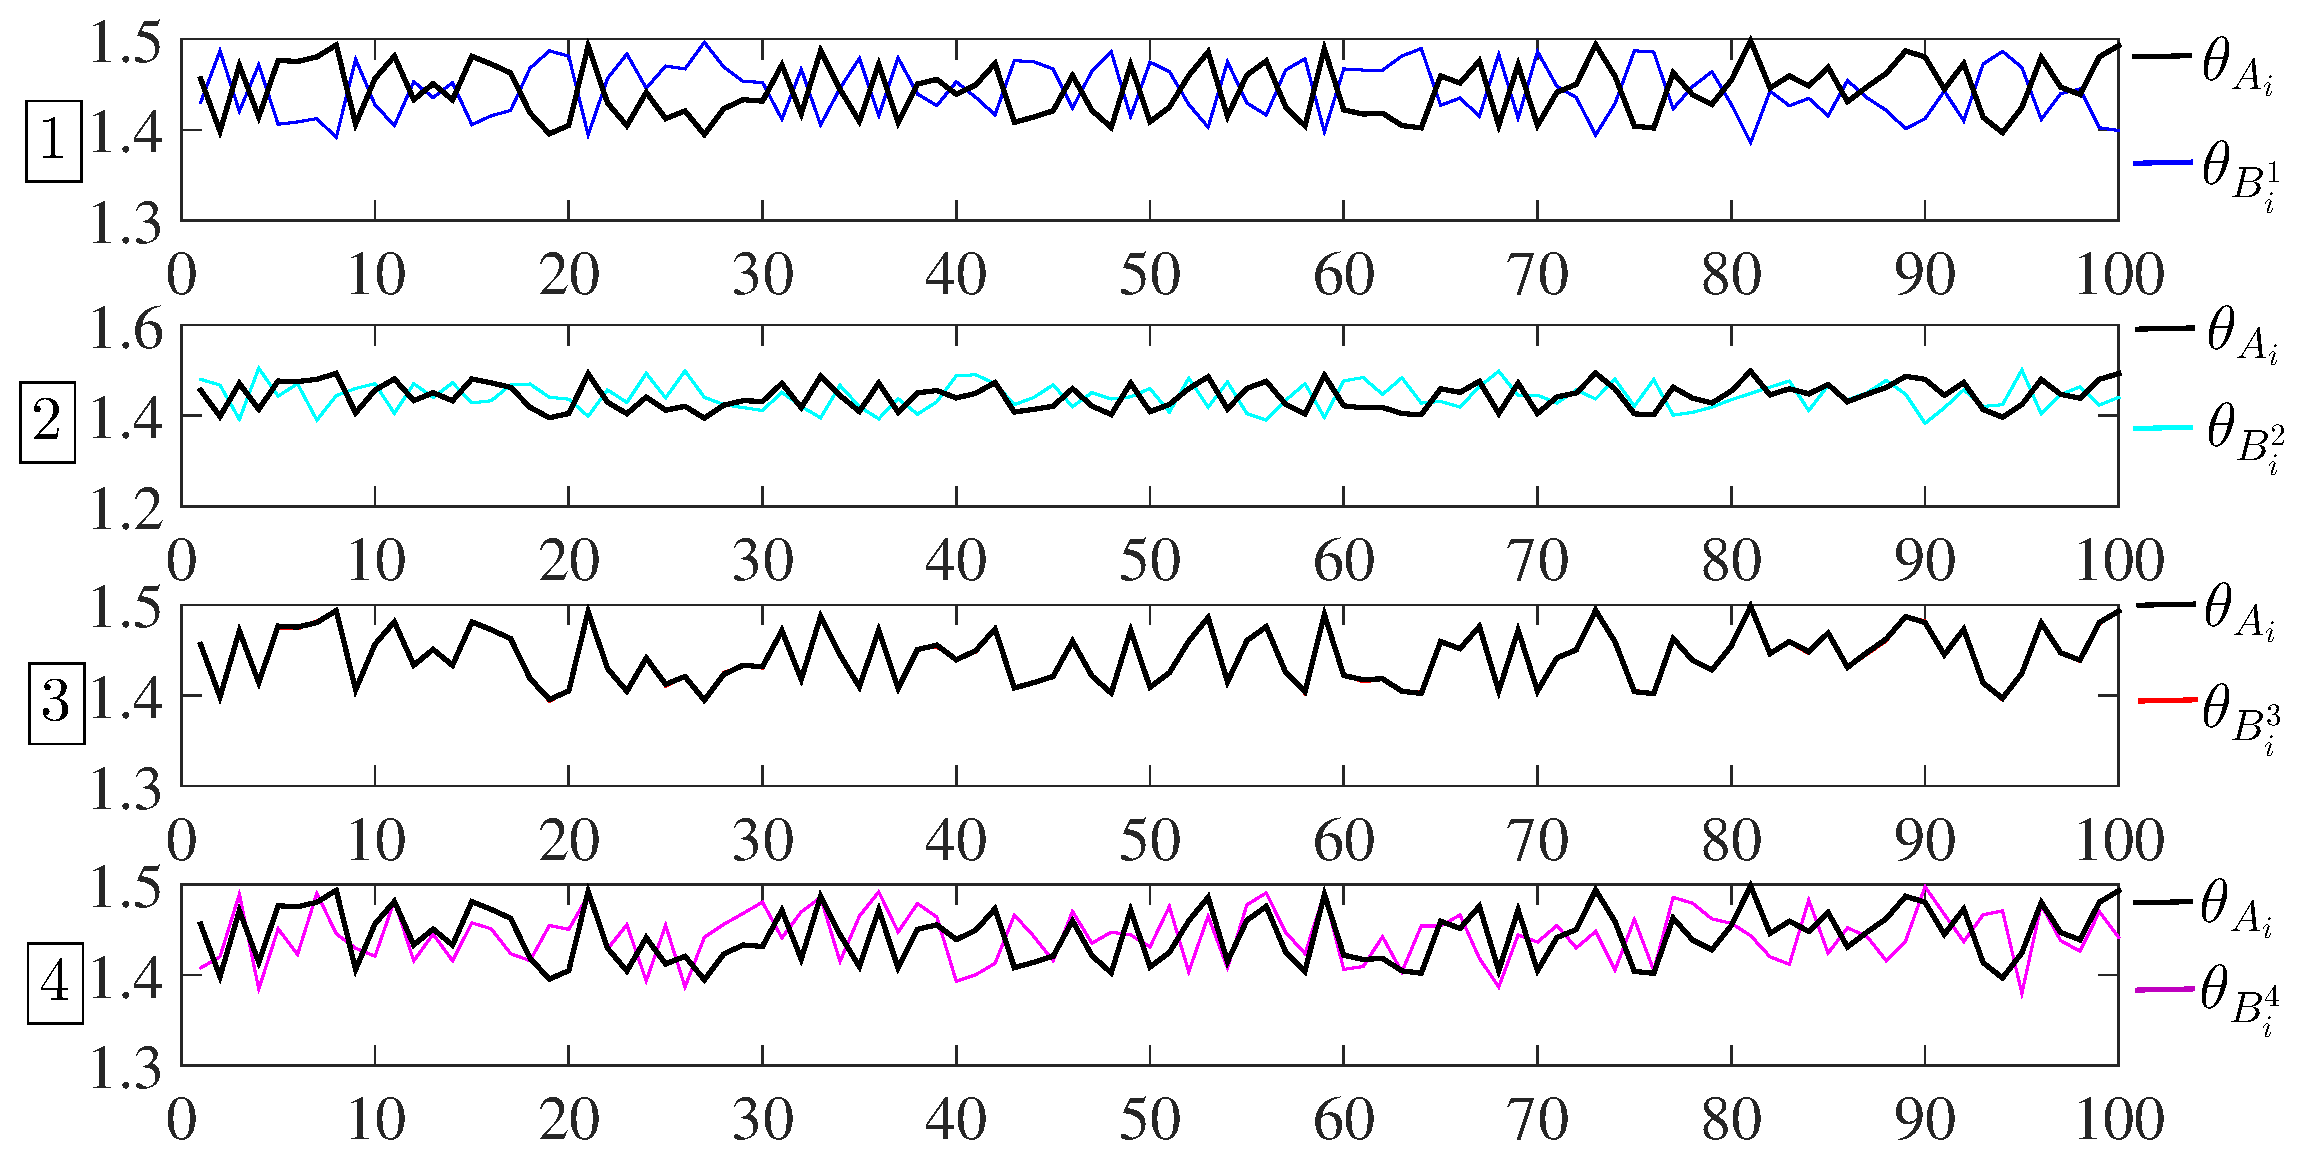
\includegraphics[width=3.2in]{fig2.eps}
\caption{
Calculated four pairs of rotational angles $(\theta_{A_{i}},\theta_{B_{i}^{k}}) (k=1,2,3,4)$  respectively from 100 measurements
}
\label{fig2}
\end{figure}
\end{center}

\begin{center}
\begin{figure}[htbp]
\centering
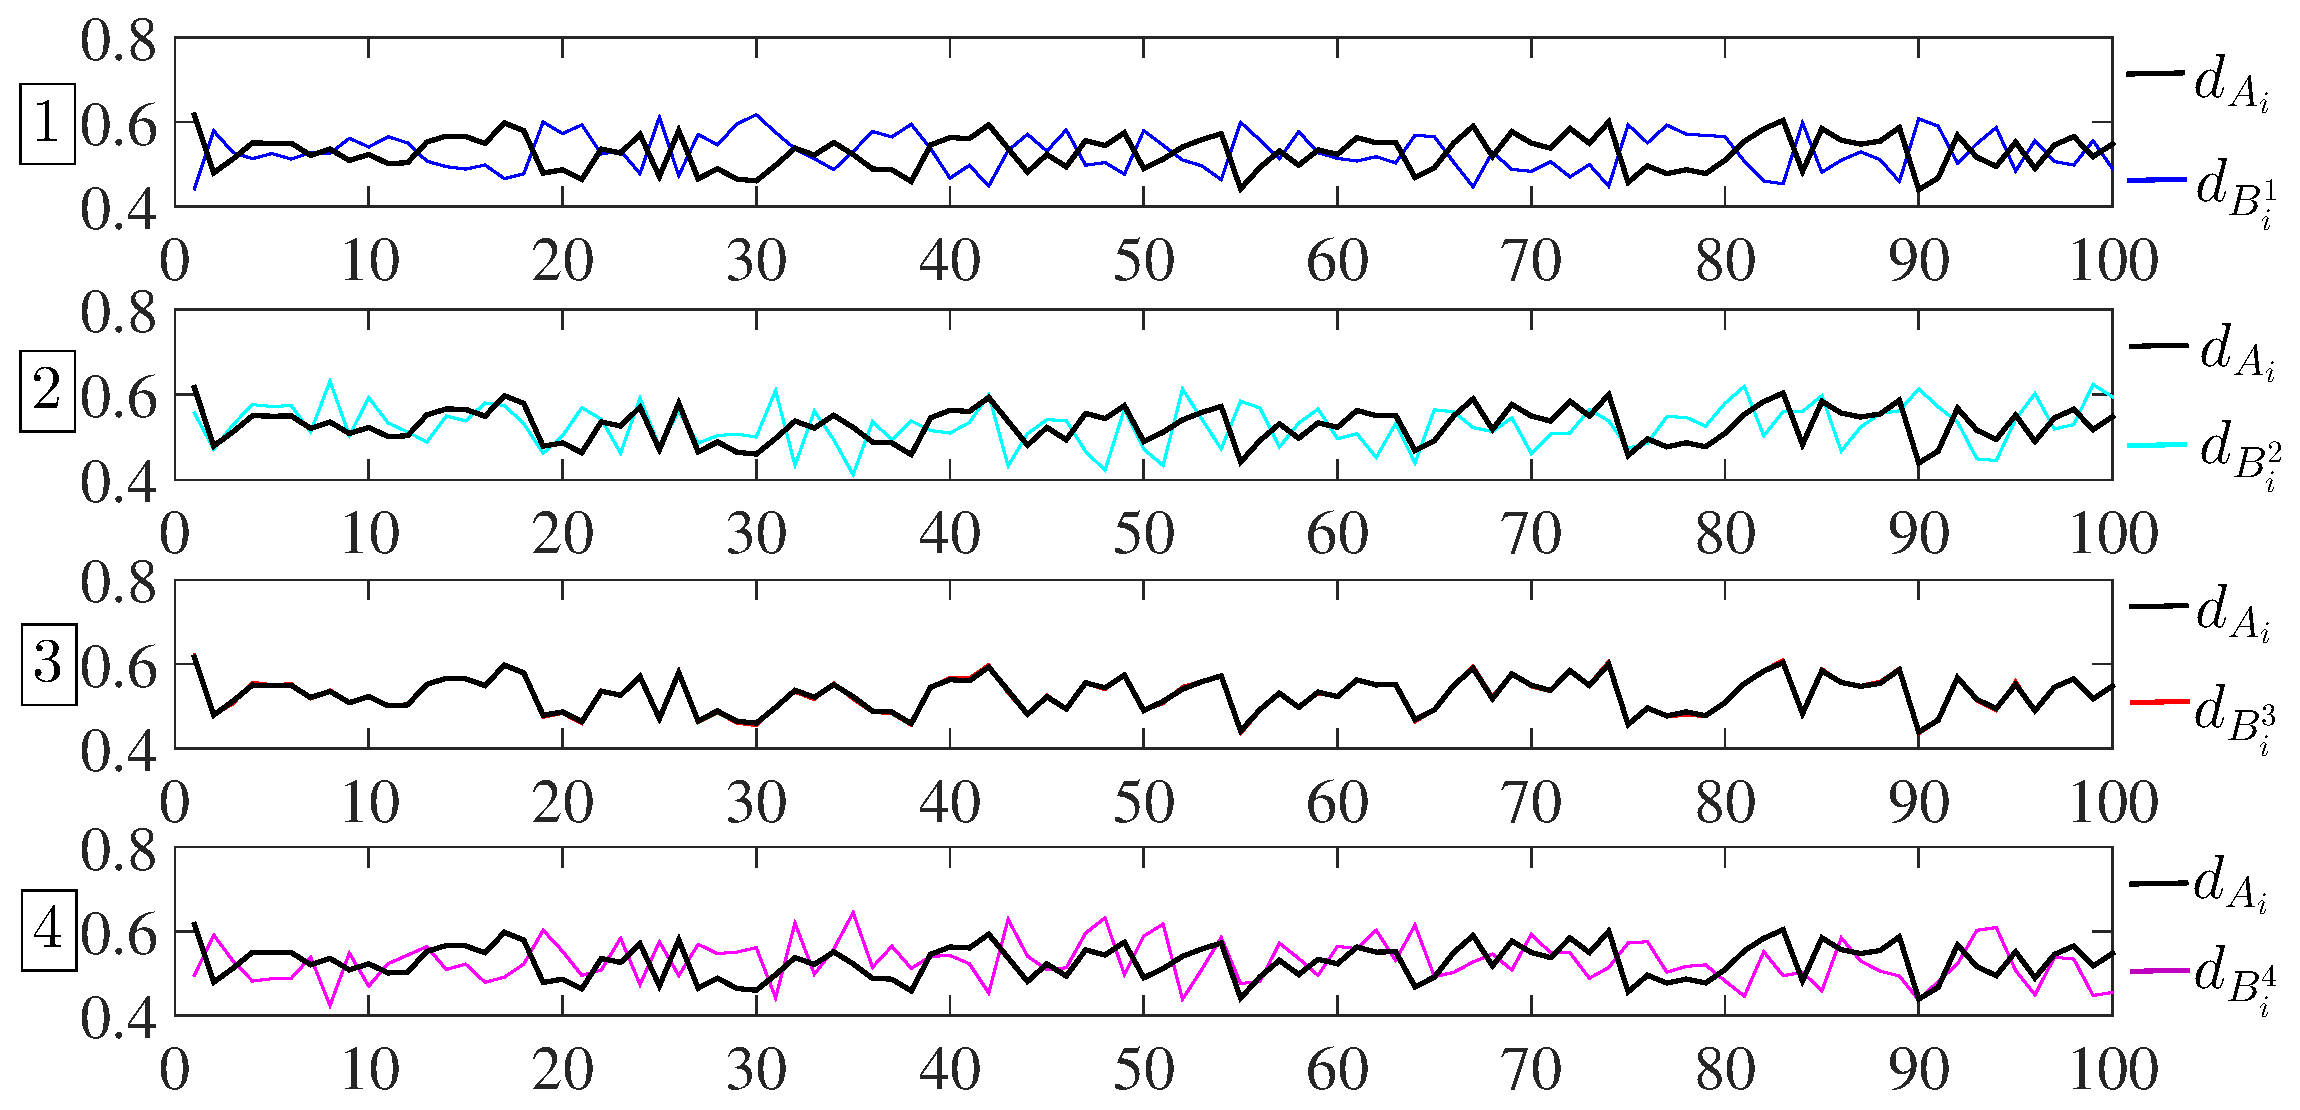
\includegraphics[width=3.2in]{fig3.eps}
\caption{
Calculated four pairs of translational displacement  $(d_{A_{i}},d_{B_{i}^{k}}) (k=1,2,3,4)$  respectively from 100 measurements
}
\label{fig3}
\end{figure}
\end{center}

\begin{center}
\begin{figure}[htbp]
\centering
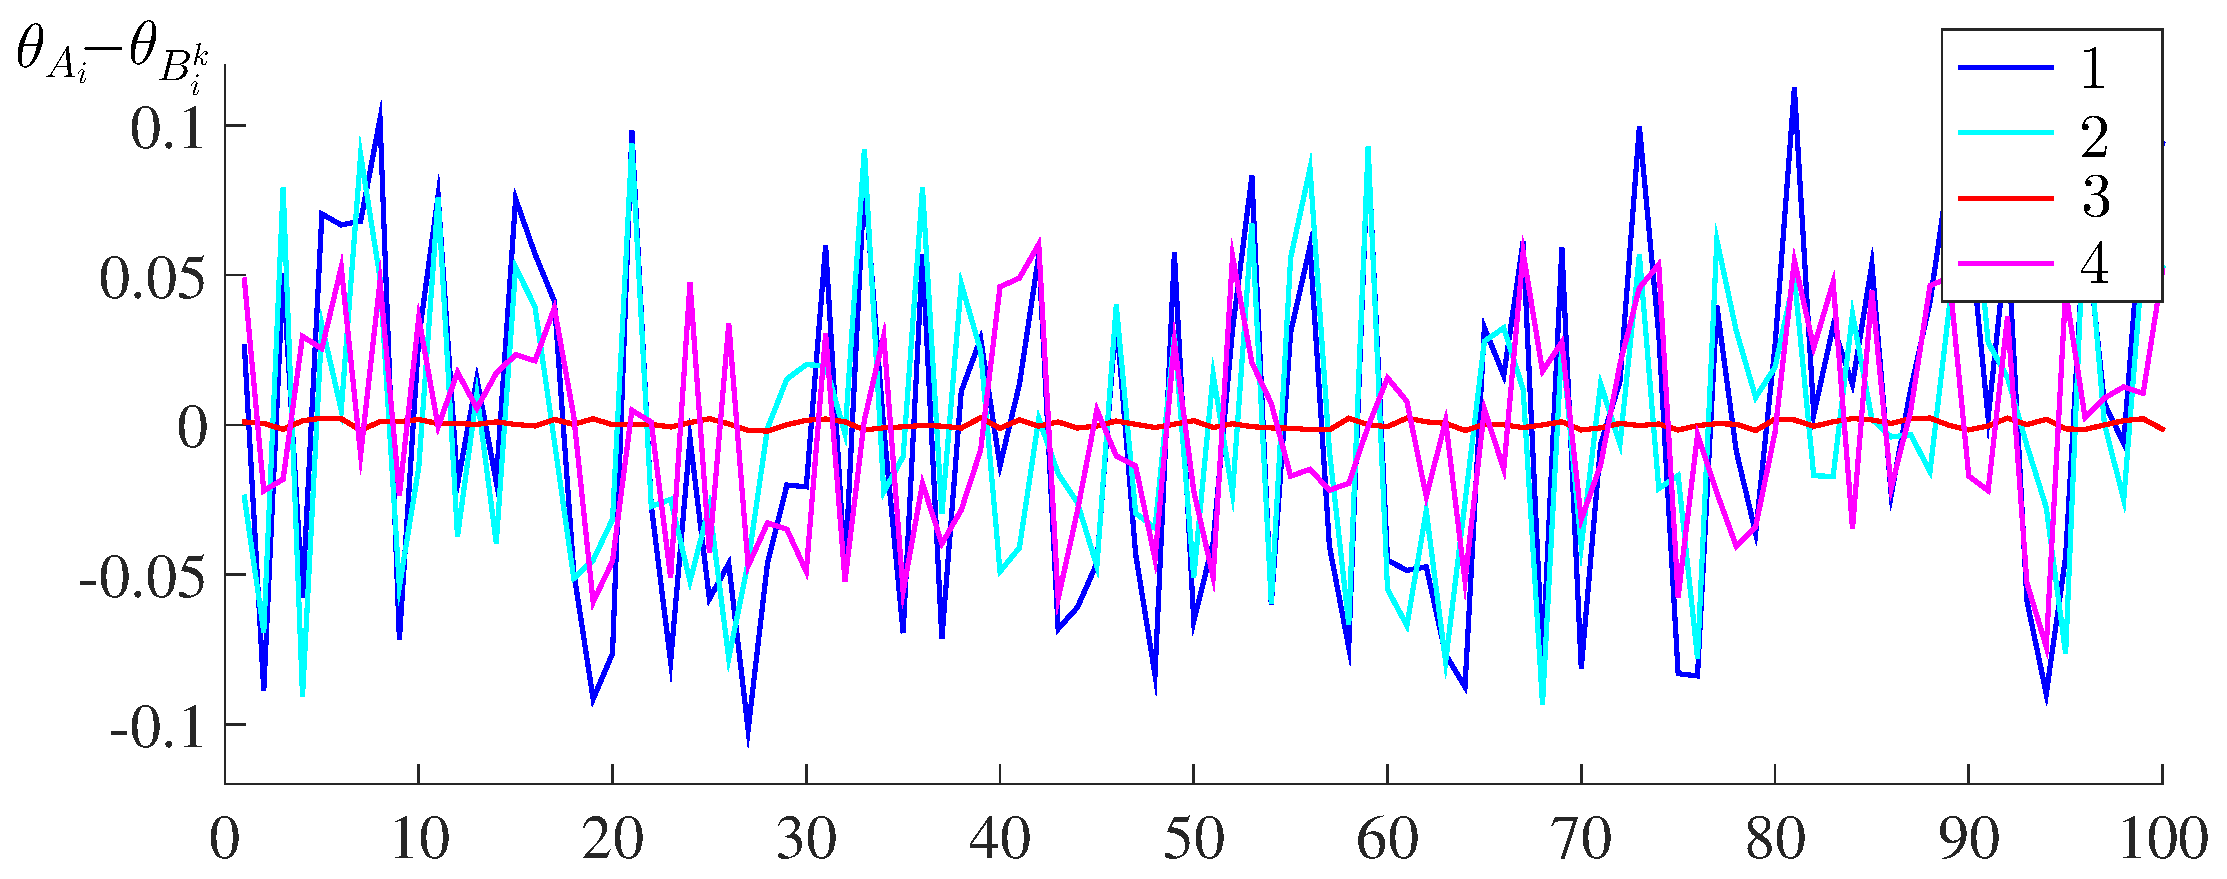
\includegraphics[width=3.2in]{fig4.eps}
\caption{
Calculated rotational angle deviation $\theta_{A_{i}} - \theta_{B_{i}^{k}} (k=1,2,3,4)$ from Fig.~\ref{fig2}
}
\label{fig4}
\end{figure}
\end{center}

\begin{center}
\begin{figure}[htbp]
\centering
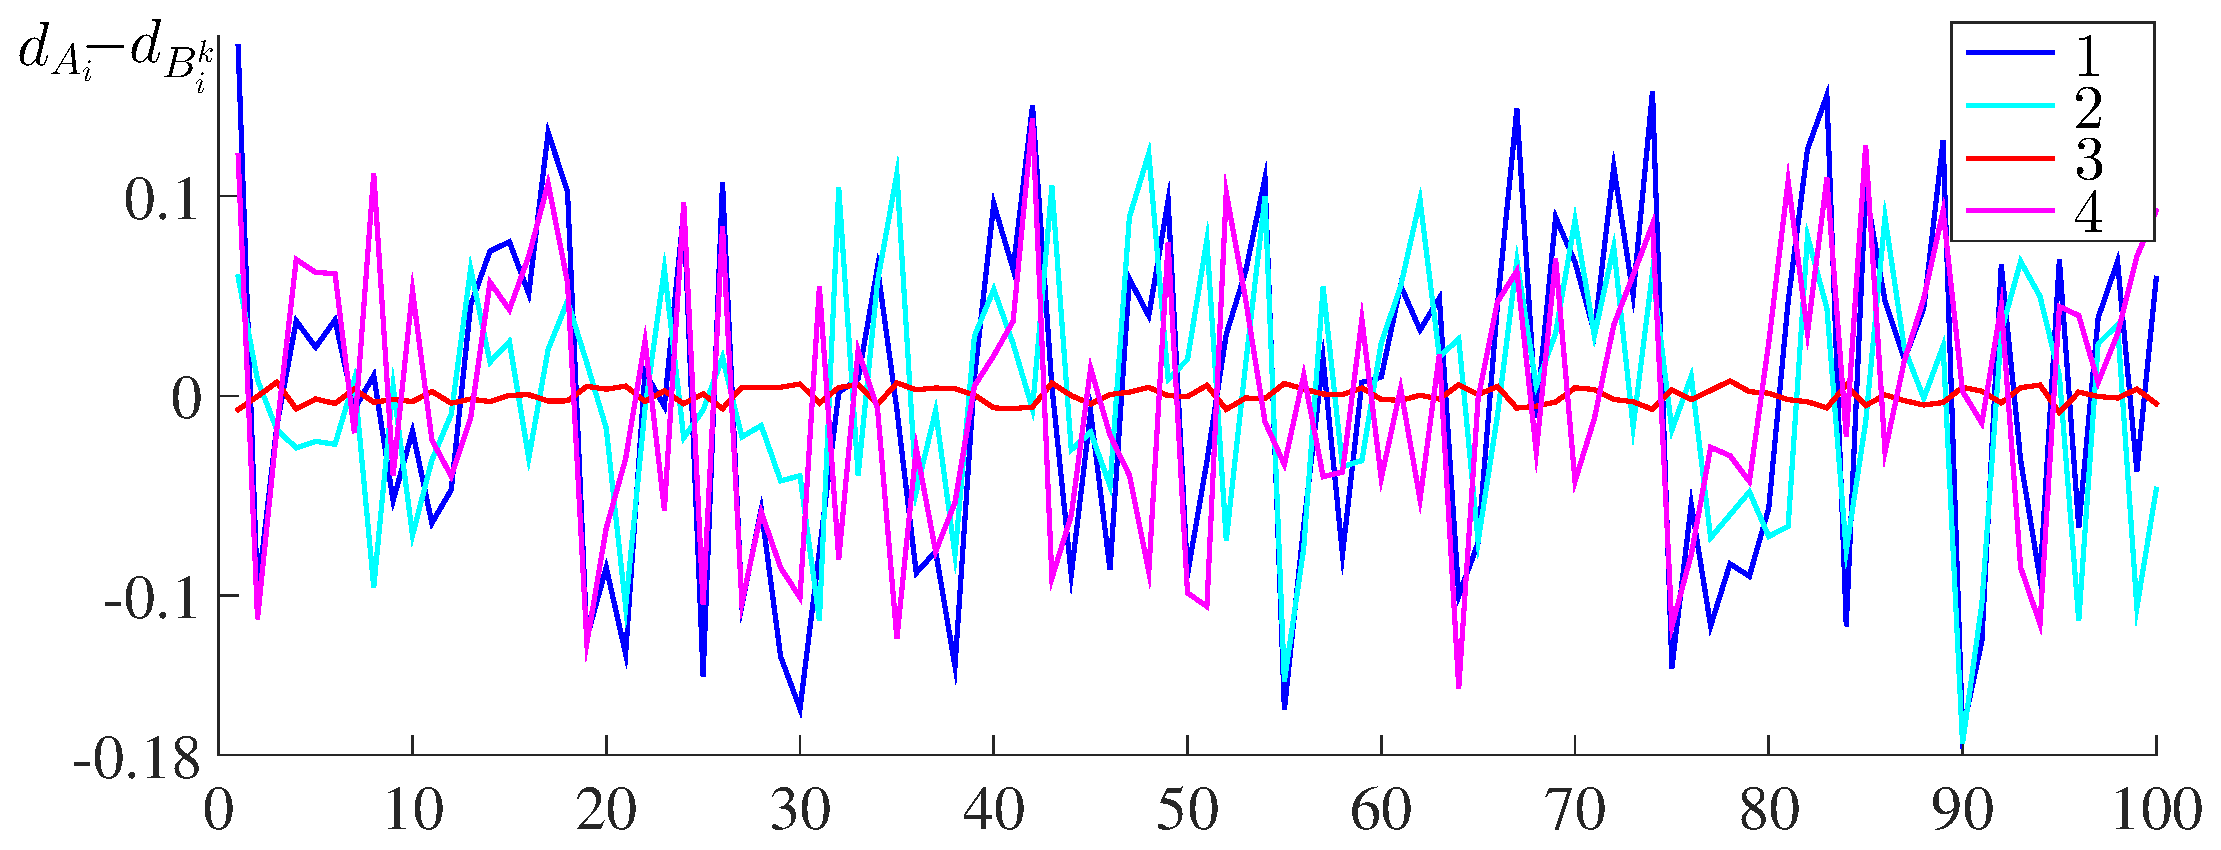
\includegraphics[width=3.2in]{fig5.eps}
\caption{
Calculated translational deviation $d_{A_{i}} - d_{B_{i}^{k}} (k=1,2,3,4)$ from Fig.~\ref{fig3}
}
\label{fig5}
\end{figure}
\end{center}

\begin{center}
\begin{figure}[htbp]
\centering
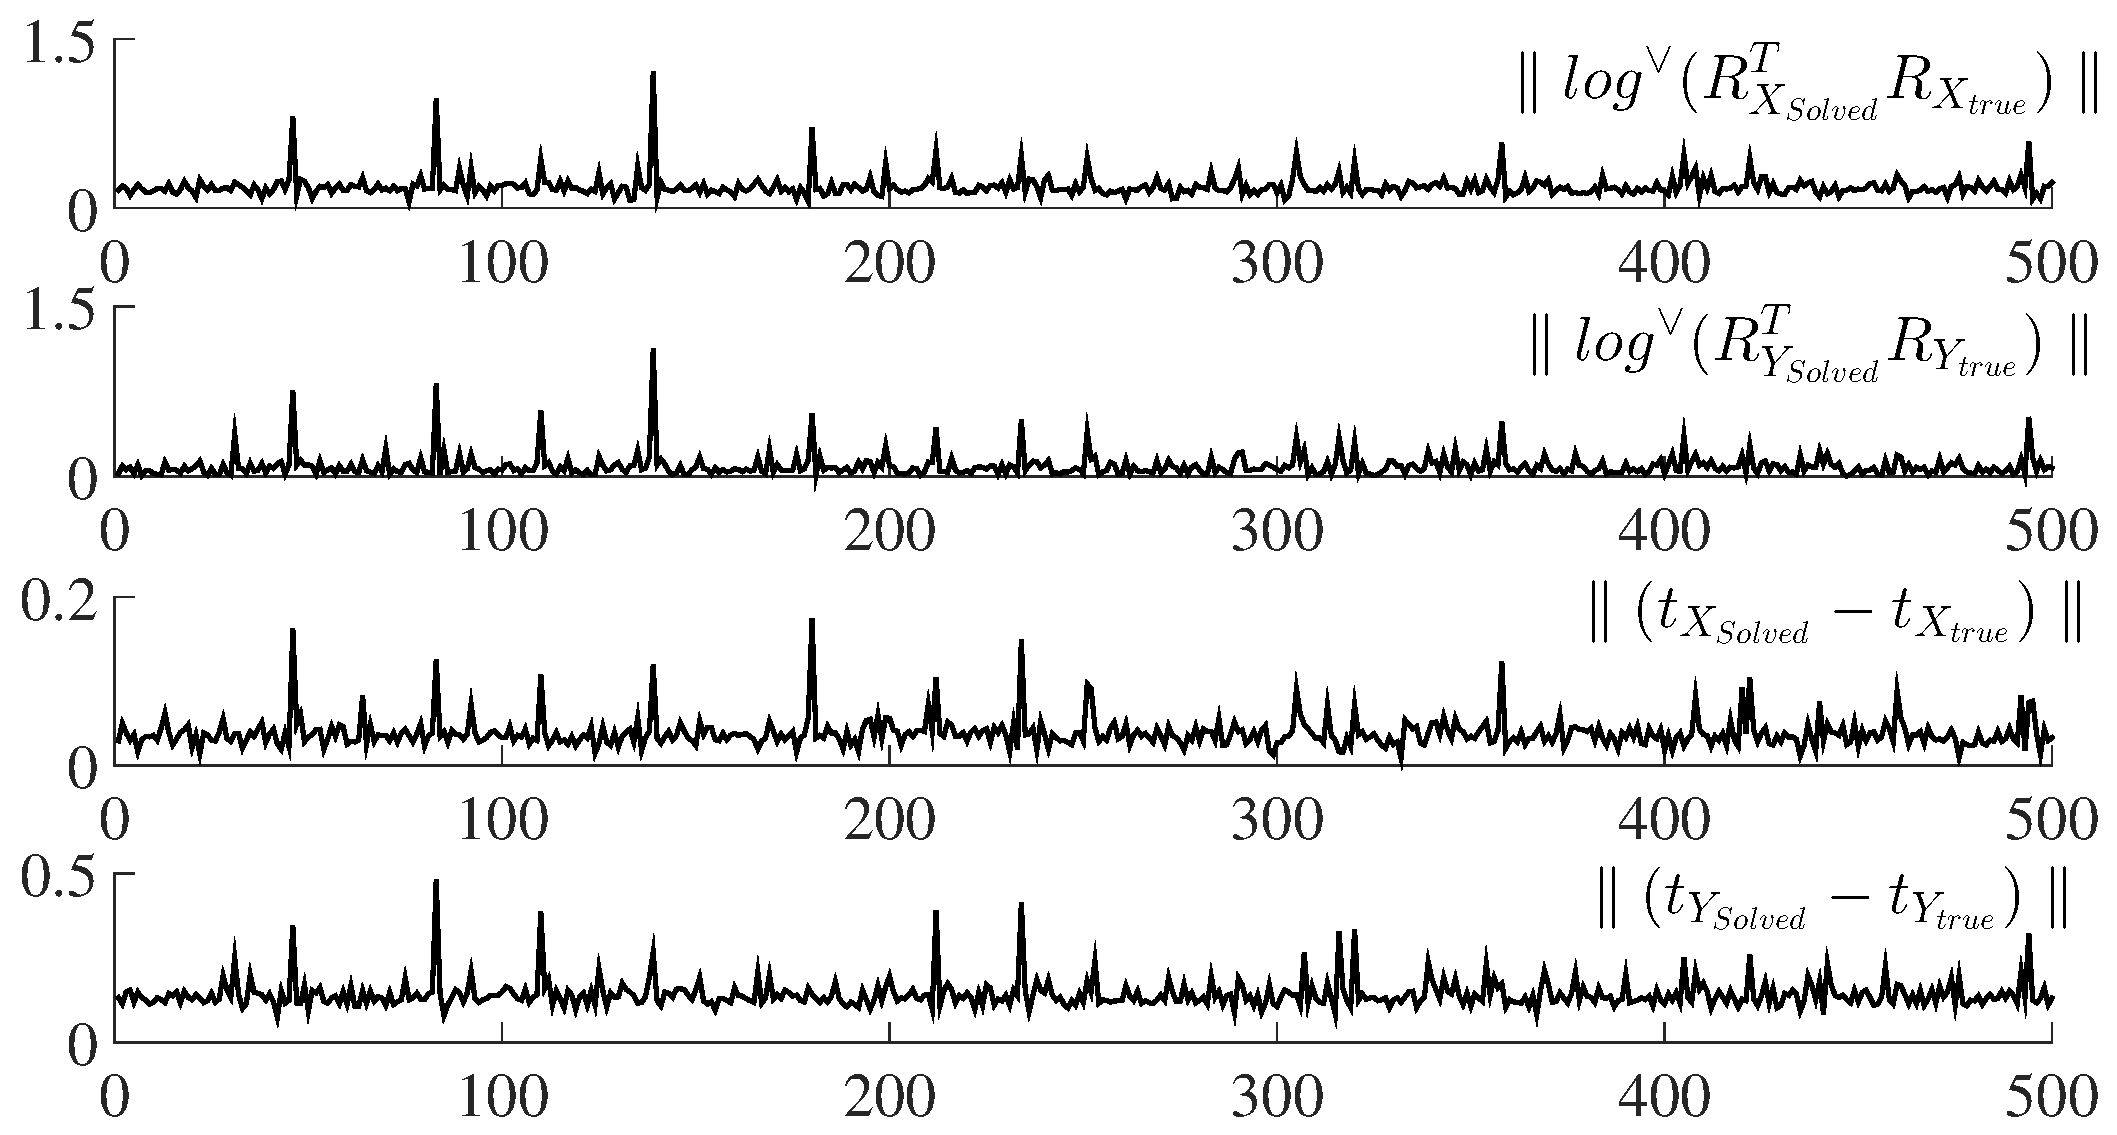
\includegraphics[width=3.2in]{fig6.eps}
\caption{
Solution error with increasing pairs $(A_{i},B_{i}^{k})$ from 1 measurements to 500 measurements
}
\label{fig6}
\end{figure}
\end{center}

\subsection{Results of solution without known correspondence}
As shown in Fig.~\ref{fig7}, the data streams of $A$ were shifted by 10 units. The maximum of cross correlation can be used to find the corresponding shift, which is -10 shown in Fig.~\ref{fig8}, representing the data stream of $B_{i}^{k}$ has been shifted by -10 units respective to ${A_{i}}$ . Therefore, we shift the data stream inversely to recover the correspondence for finding a correct solution satisfying Euclidean-Group Invariants.

\begin{center}
\begin{figure}[htbp]
\centering
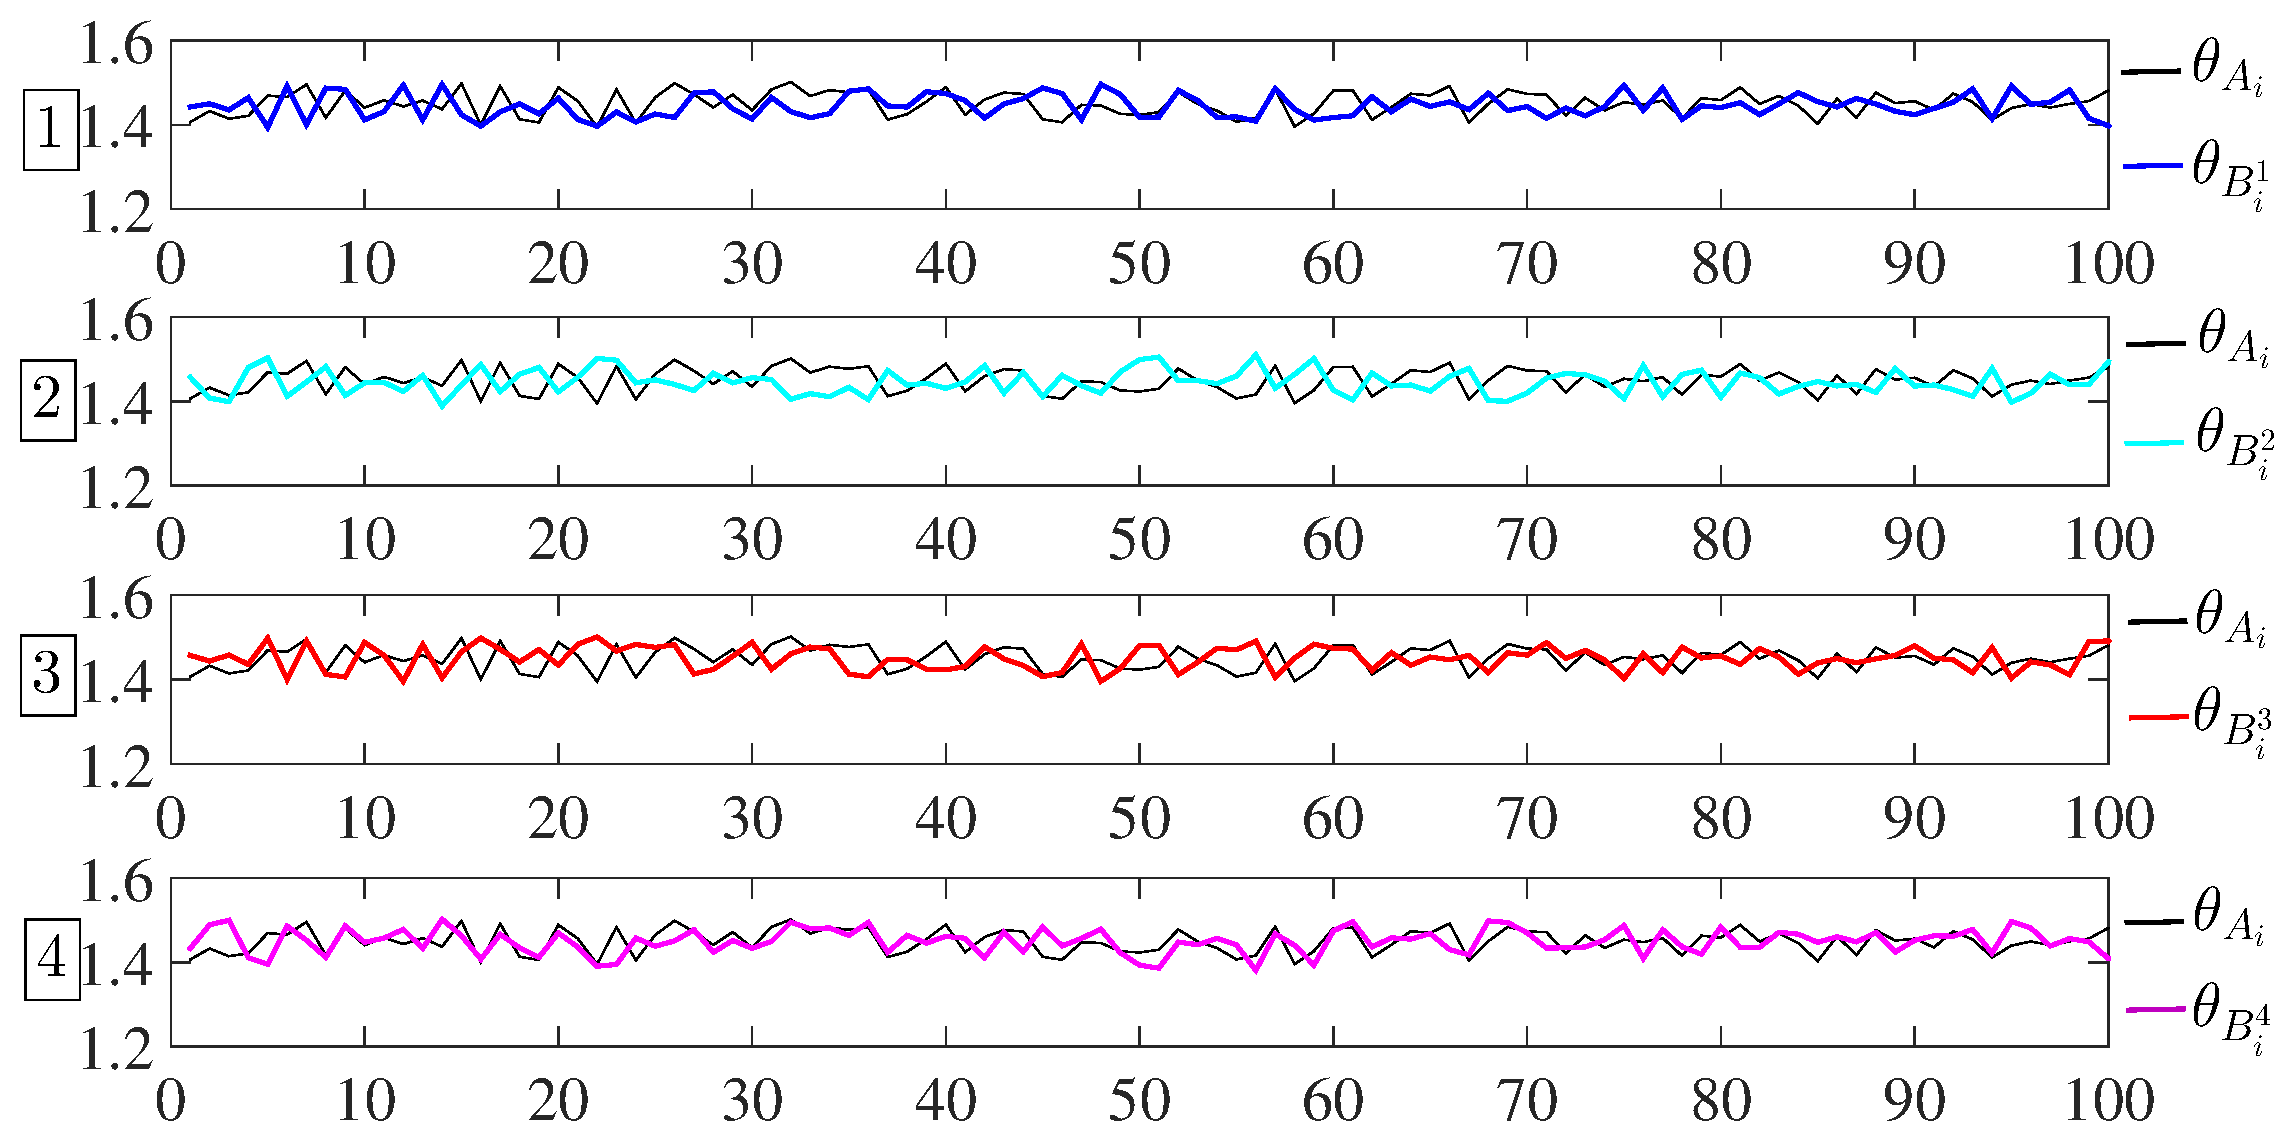
\includegraphics[width=3.2in]{fig7.eps}
\caption{
Shifted Data Streams of $A$ and calculated $B_{i}^{k}$.
}
\label{fig7}
\end{figure}
\end{center}
\begin{center}

\begin{figure}[htbp]
\centering
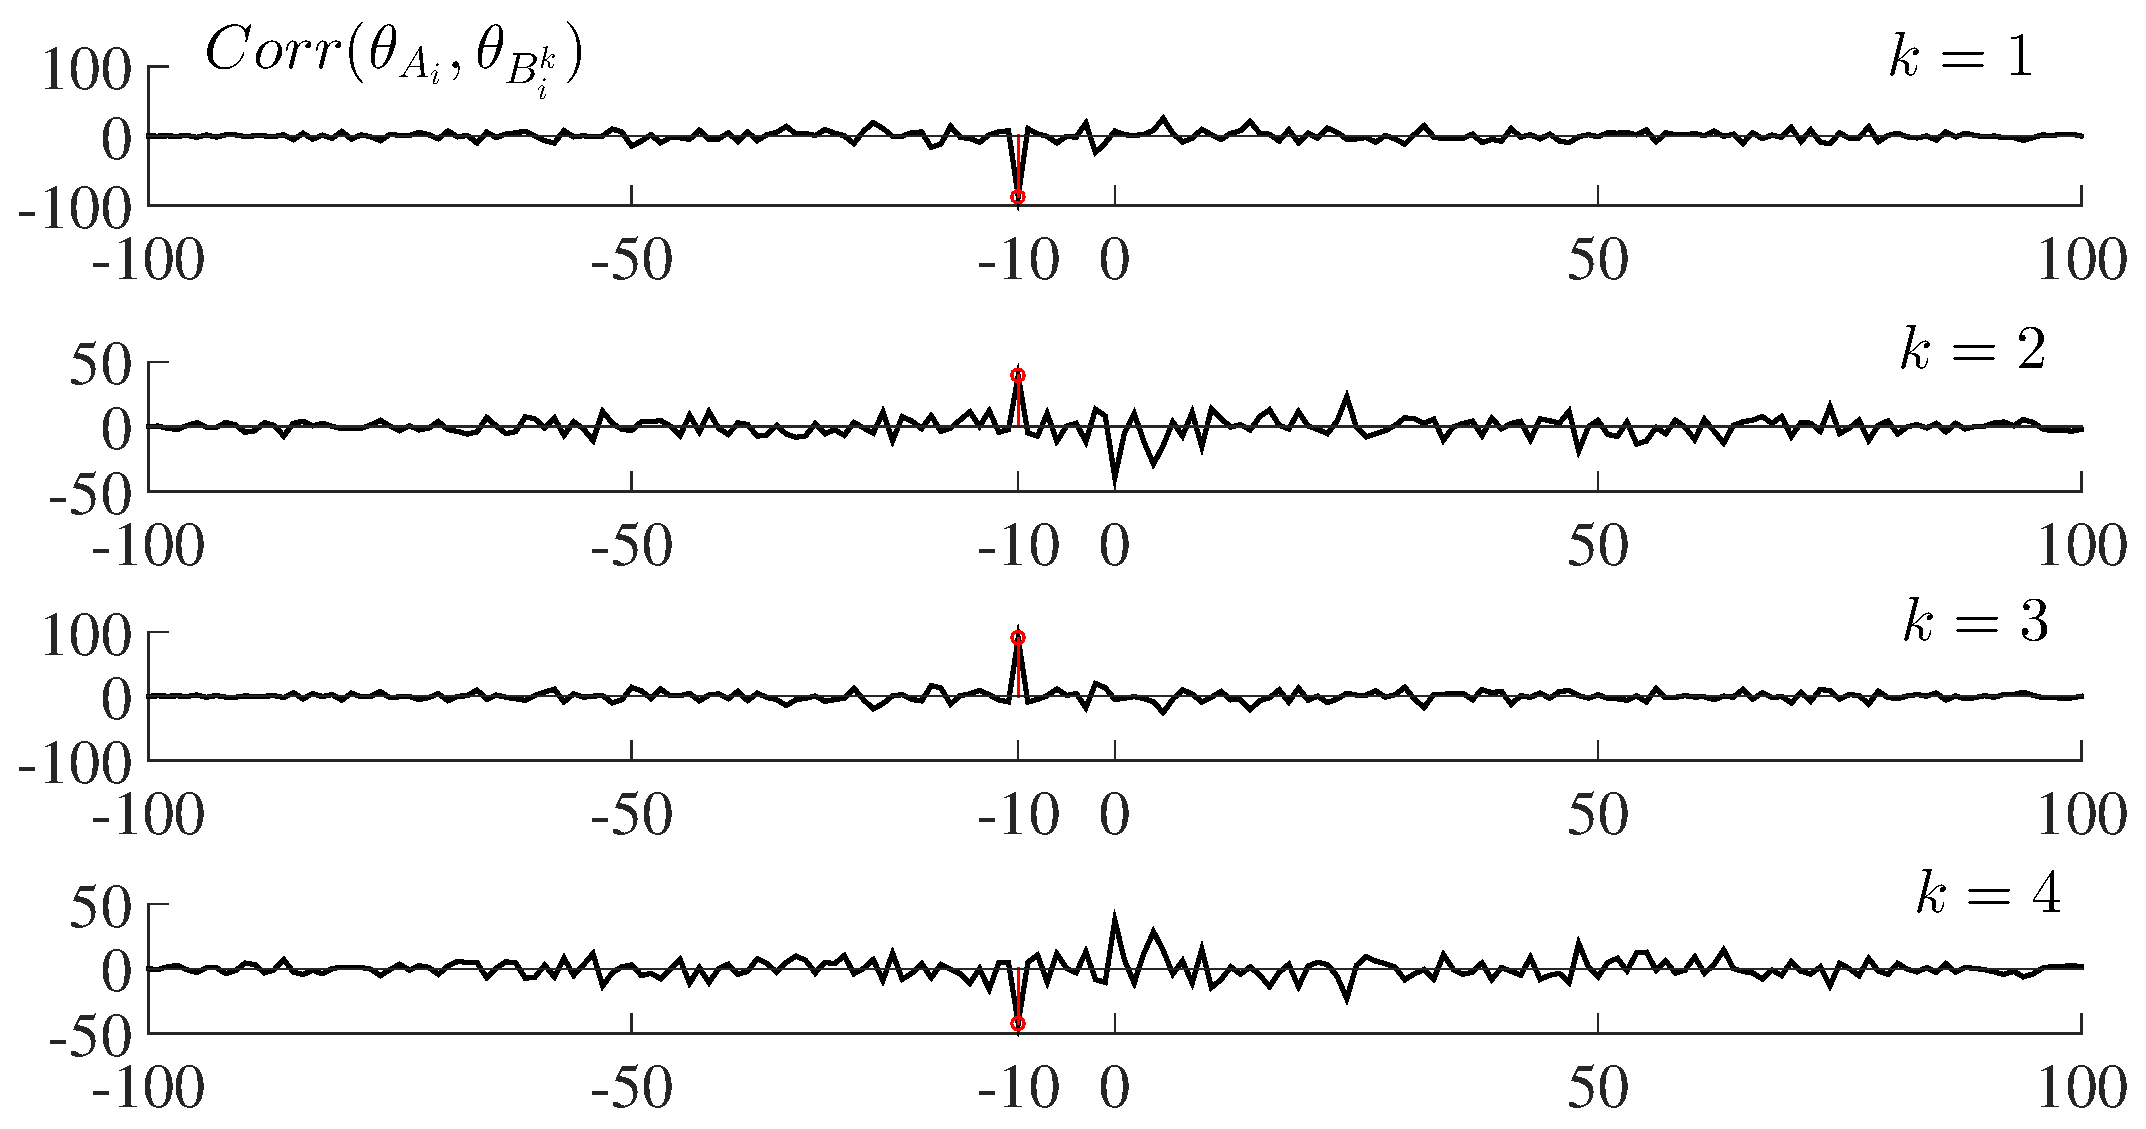
\includegraphics[width=3.2in]{fig8.eps}
\caption{
The cross correlation of data streams of $(A_{i},B_{i}^{k})$ respectively.
}
\label{fig8}
\end{figure}
\end{center}

\section{Conclusions}
\label{sect5}

Conclusions
%\section{Conclusion}
% conference papers do not normally have an appendix

% use section* for acknowledgment
\section*{Acknowledgment}

acknowledgement
% optional entry into table of contents (if used)
%\addcontentsline{toc}{section}{Acknowledgment}


% trigger a \newpage just before the given reference
% number - used to balance the columns on the last page
% adjust value as needed - may need to be readjusted if
% the document is modified later
%\IEEEtriggeratref{8}
% The "triggered" command can be changed if desired:
%\IEEEtriggercmd{\enlargethispage{-5in}}

% references section

\bibliographystyle{IEEEtran}
\bibliography{IEEEabrv,bibIEEEfull}
%\begin{thebibliography}{1}
%
%
%\end{thebibliography}

\end{document}
